
\documentclass[11pt,reqno,twoside]{article}
\usepackage{ dsfont }
\usepackage{float}
% >>>> DO NOT EDIT THIS FILE
% If you *must* add or change a macro, please email fkoh@caltech.edu

%=================================================
% Basics
%=================================================

\usepackage{fixltx2e} % Makes \( \) equation style robust, among other
                      % things. Must be the first package.


% Makes ligatured fonts searchable and copyable in pdf readers
\usepackage{cmap} % Load before fontenc
\usepackage[spanish]{babel}

% Always include these font encodings in your document
% unless you have a very good reason.
\usepackage[T1]{fontenc}
\usepackage[utf8]{inputenc}

\usepackage{verbatim}

%=====================================
% Look & feel
%=====================================

% Allows for manual space setting
\usepackage{setspace}

%=============
% Fonts
%=============

\usepackage{lmodern} % Improved version of computer modern
\usepackage[scale=0.88]{tgheros} % Helvetica clone for sans serif font


\newcommand\hmmax{2} % Default is 3.
\newcommand\bmmax{2} % Default is 4.

\usepackage{bm} % boldmath must be called after the package
\providecommand{\mathbold}[1]{\bm{#1}}

%=============
% AMS Packages and fonts
%=============
\usepackage{amsmath,amsbsy,amsgen,amscd,amsthm,amsfonts,amssymb}

%=============
% Margins and paper size
%=============
\usepackage[centering,top=1.5in,bottom=1.2in,left=1.4in,right=1.4in]{geometry}

%=============
% Title setup
%=============
\usepackage{titling}
%\usepackage{nopageno}
\setlength{\droptitle}{-7.5em}

\pretitle{\noindent\rule{0.85\linewidth}{0.2mm}\par%
  \begin{raggedright}\LARGE\sffamily}
\posttitle{\par\end{raggedright}%
\noindent%
\rule{0.85\linewidth}{0.5mm}\par}

\preauthor{\noindent\vspace{0.5em}%
  \sffamily\begin{tabular}[t]{ll}}
  \postauthor{\end{tabular}\par\thispagestyle{plain}}

\predate{\noindent%
  \small\sffamily\itshape\begin{tabular}[t]{l}%
    EST-25134, Primavera 2021 \\ %
    Dr.\ Alfredo Garbuno Iñigo \\ %
  }
  \postdate{
  \end{tabular}\par}

%=============
% Section headings
%=============
\usepackage[sf,bf,compact]{titlesec}

%=============
% Tables and lists
%=============
\usepackage{booktabs,longtable,tabu} % Nice tables
\setlength{\tabulinesep}{1mm}
\usepackage[font=small,margin=10pt,labelfont={sf,bf},labelsep={space}]{caption}


\usepackage{enumitem}
\setitemize{itemsep=0pt}
\setenumerate{itemsep=0pt}
\setlist{labelindent=\parindent,%  % Recommended by enumitem package
  font=\sffamily}


%=============
% Hyperlink colors
%=============
\usepackage[usenames,dvipsnames]{xcolor}
\definecolor{dark-gray}{gray}{0.3}
\definecolor{dkgray}{rgb}{.4,.4,.4}
\definecolor{dkblue}{rgb}{0,0,.5}
\definecolor{medblue}{rgb}{0,0,.75}
\definecolor{rust}{rgb}{0.5,0.1,0.1}

\usepackage{url}
\usepackage[colorlinks=true]{hyperref}
\hypersetup{linkcolor=dkblue}
\hypersetup{citecolor=rust}
\hypersetup{urlcolor=rust}
\usepackage[spanish, capitalise]{cleveref}
\usepackage{autonum}
%=============
% Microtype
%=============
\usepackage[final]{microtype}

%=============
% Theorems, etc.
%=============
\newtheoremstyle{myThm} % name
    {\topsep}                    % Space above
    {\topsep}                    % Space below
    {\itshape}                   % Body font
    {}                           % Indent amount
    {\sffamily\bfseries}                   % Theorem head font
    {.}                          % Punctuation after theorem head
    {.5em}                       % Space after theorem head
    {}  % Theorem head spec (can be left empty, meaning ‘normal’)

\newtheoremstyle{myRem} % name
    {\topsep}                    % Space above
    {\topsep}                    % Space below
    {}                   % Body font
    {}                           % Indent amount
    {\sffamily}                   % Theorem head font
    {.}                          % Punctuation after theorem head
    {.5em}                       % Space after theorem head
    {}  % Theorem head spec (can be left empty, meaning ‘normal’)

\newtheoremstyle{myDef} % name
    {\topsep}                    % Space above
    {\topsep}                    % Space below
    {}                   % Body font
    {}                           % Indent amount
    {\sffamily\bfseries}                   % Theorem head font
    {.}                          % Punctuation after theorem head
    {.5em}                       % Space after theorem head
    {}  % Theorem head spec (can be left empty, meaning ‘normal’)

\theoremstyle{myThm}
\newtheorem{theorem}{Teorema}[section]
\newtheorem{lemma}[theorem]{Lemma}
\newtheorem{proposition}[theorem]{Proposition}
\newtheorem{corollary}[theorem]{Corollary}
\newtheorem{fact}[theorem]{Fact}

\theoremstyle{myRem}
\newtheorem{remark}[theorem]{Remark}

\theoremstyle{myDef}
\newtheorem{definition}[theorem]{Definition}
\newtheorem{example}[theorem]{Example}

%=====================
% Header
%=====================
\usepackage{fancyhdr}
\usepackage{nopageno} % Gets rid of page number at the bottom
\fancyhf{} % Clear header style
\renewcommand{\headrulewidth}{0.5pt} % remove the header rule
\pagestyle{fancy}
\fancyhead[LE,RO]{\textsf{\small \thepage}}

\setlength{\headheight}{14pt}
%=====================
% Fix delimiters
%=====================

% Fixes \left and \right spacing issues. See discussion at
% http://tex.stackexchange.com/questions/2607/spacing-around-left-and-right
\let\originalleft\left
\let\originalright\right
\renewcommand{\left}{\mathopen{}\mathclose\bgroup\originalleft}
\renewcommand{\right}{\aftergroup\egroup\originalright}

%=================================================
% Math macros
%=================================================

%=============
% Generalities
%=============
\usepackage{mathtools}
\mathtoolsset{centercolon}  % Makes := typeset correctly for definitions

%%% Equation numbering
%\numberwithin{equation}{section}

%%% Annotations
\newcommand{\notate}[1]{\textcolor{red}{\textbf{[#1]}}}

%==============
% Symbols
%==============
\let\oldphi\phi
\let\oldeps\epsilon
\let\oldemptyset\emptyset
\let\emptyset\varnothing

\renewcommand{\phi}{\varphi}
\renewcommand{\epsilon}{\varepsilon}
\newcommand{\eps}{\varepsilon}
\newcommand{\cl}{\mathrm{cl}}
\newcommand{\wto}{\rightharpoonup}
\newcommand{\wsto}{\overset{\ast}{\rightharpoonup}}
\newcommand{\wwto}{\overset{w}{\to}}
\newcommand{\wwsto}{\overset{w*}{\to}}

%==============
% Constants
%==============

% Set constants upright
\newcommand{\cnst}[1]{\mathrm{#1}}
\newcommand{\econst}{\mathrm{e}}
\newcommand{\rd}{\mathrm{d}}
\newcommand{\dist}{\mathrm{dist}}

\newcommand{\zerovct}{\vct{0}} % Zero vector
\newcommand{\Id}{\mathbf{I}} % Identity matrix
\newcommand{\onemtx}{\bm{1}}
\newcommand{\zeromtx}{\bm{0}}

%==============
% Sets
%==============
\providecommand{\mathbbm}{\mathbb} % In case we don't load bbm

% Reals, complex, naturals, integers, field
\newcommand{\R}{\mathbbm{R}}
\newcommand{\C}{\mathbbm{C}}
\newcommand{\N}{\mathbbm{N}}
\newcommand{\Z}{\mathbbm{Z}}
\newcommand{\F}{\mathbbm{F}}

%==============
% Probability
%==============
\newcommand{\Prob}{\operatorname{\mathbbm{P}}}
\newcommand{\Expect}{\operatorname{\mathbb{E}}}
\newcommand{\D}{\operatorname{\mathcal{D}}}

%==============
% Vectors and matrices
%==============
\newcommand{\vct}[1]{\mathbold{#1}}
\newcommand{\mtx}[1]{\mathbold{#1}}

%=============
% Operators
%=============
\newcommand{\B}{\mathcal{B}}
\newcommand{\op}[1]{\mathbold{#1}} 

\title{Clase 10:               % UPDATE LECTURE NUMBER
    Boosting}	% UPDATE TITLE

\author{%
  Responsable:& Mariana Pérez-Cong Sánchez % >>>>> SCRIBE NAME(S)
}

\begin{document}
\maketitle 

\section{Introducción}
\label{sec:introduction}
\begin{itemize}
    \item Quisieramos ver una generalizacion sobre los predictores lineales
    \item  Que sean capaces de atacar el compromiso de sesgo y varianza.
    \begin{itemize}
        \item Mayor complejidad $\Rightarrow$ error de aproximación pequeño
        
    \end{itemize}
    \item Boosting nos permite controlar este compromiso por medio de un parámetro. Empieza con un modelo sencillo pero gana complejidad en el proceso de aprendizaje.
    \item Vamos a ver \textbf{Ada Boost} (Adaptative Boosting): combina predicciones de manera lineal.
    
\end{itemize}


\section{Capacidad de aprendizaje Débil}
Tenemos:
\begin{itemize}
    \item PAC con $m_H(\epsilon, \delta)$
    \item Teorema fundamental de Aprendizaje Estadístico $\rightarrow$ ERM
    \item ¿Existe un algoritmo eficiente con un error ligeramente mejor que lanzar una moneda?
\end{itemize}
\\
\textbf{Definición:}\\
Un algoritmo A es $\gamma-débil$ para H si $\exists m_H:(0,1)\rightarrow \N$ tal que $\forall \delta \in (0,1)$, D y $f: X \rightarrow \{ \pm 1\}$ y si se mantiene la hipótesis de realizabiladidad,entonces con $m> m_H(\delta)$ iid de D, el algoritmo regresa un candidato $h \in H$ tal que con probabilidad mayor o igual a $1-\delta$, $L_D(h)\leq \frac{1}{2}-\gamma$
\begin{itemize}
    \item Decimos que H es $\gamma- débil$ si existe un algoritmo $\gamma-débil$ para dicha clase
\end{itemize}
\\
\textbf{Ejemplo:} Sea $X=\R$ y H los clasificadores en tres partes:
\[H= \{ h_{\theta_1, \theta_2,b}: \theta_1, \theta_2 \in \R, \theta_1 < \theta_2 , b \in \{ \pm 1\}\}\]
\[h_{\theta_1, \theta_2,b}(x)= \begin{cases}-b \qquad \text{si }  x<\theta \text{ o } x>\theta_2\\-b \qquad \text{si } x\in [\theta_1, \theta_2]\end{cases} \]
Sea $B=\{f:f(x)=signo(x-\theta) \cdot b : \theta \in \R, b \in \{\pm 1\}\}$. Veremos que $ERM_b$ es $\gamma-debil$ para H con $\gamma=1/2$. $\exists h \in B$ que tendrá un error de clasificacion $Ld(h)<\frac{1}{3}$\\
$VCdim(B)=2 \Rightarrow m_H(\gamma) \geq \frac{log(1/\gamma)}{\epsilon}$ (módulo una constante).

Entonces, Con prob $ \geq 1-\delta$, ERM tiene un error de generalizacion $\leq 1/3 + \epsilon. $\\ Si consideramos $\epsilon =1/12$ $\Rightarrow 1/3+1/12=1/2-1/12$\\
$\therefore ERM_b$  es $\gamma-debil$

\subsection{Implementacion}
Sea $X= \R^d$; $H_{DS}=\{g:g(x)=signo(\theta-x_i), x \in \R ^d, \theta \in \R, i=\{1,..., d\}\}$
Sea $S=\{(x_i, y_i)\}_{i=1}^{m}$.\\ Vamos a ver cómo minimizar $L_s(h)$y cómo se pueden usar estos predictores débiles para Ada Boost.

Sea $\D$ un vector de probabilidades en $\R^m$ ($D_i \geq 0, \sum \D_i=1$). El modelo recibe $\D, S$ y regresa un predictor $h:X \rightarrow\{\pm 1\}$, donde h minimiza el riesgo con respecto a $\D$
\[L_{\D}(h)=\sum_{i=1}^{m} \D i \mathds{1}_{[h(x^{(i)}) \neq y^{(i)} ]}\]
$\forall h\in H_{DS}$ es $h=h(\theta,i)$ Entonces queremos minimizar:
\[\min_j \min_{\theta} \left( \sum_{i:y^{(i)}=1} \D_i \ \mathds{1}_{[x_j^{(i)}>\theta]}  + \sum_{i: y^{(i)}=-1} \D_i \ \mathds{1}_{[x_j^{(i)}<\theta]}\right)\]
Si consideramos fija j, podemos ordenar:
\[x_j^{(1)} \leq ... \leq x_j^{(m)}\]
\[\Theta_j = \left \{ \frac{x_j^{(i)}+x_j^{(i+1)}}{2}: i \in {1,..,m-1} \right \} \cup \left \{ x_j^{(1)}-1 , x_j^{(m)}+1 \right\}\]
Como $\forall \theta \in \R \quad \exists \theta ' \in \Theta_j$ que realiza las mismas predicciones, en lugar de optimizar $\R$, optimimizamos $\Theta_j$

\section{Ada Boost}
$S={(x^{(i)}, y^{(i)})}_{i=1}^{m}$ donde $y^{(i)}=f(x^{(i)})$.\\
Al tiempo t:
\begin{enumerate}
    \item Definimos una distribución sobre S $\D^{(t)} \in \R^{m}_+$
    \item Utilizamos un algoritmo débil con $S, \D^{(t)}$. Obtenemos $h_t$ con error
    \[\epsilon := L_{D^{(t)}} (h_t) \leq 1/2 -\gamma\]
    Con prob $\geq 1- \delta$
    \item Asignamos una contribución a $h_t$ con $w_t= \frac{1}{2} log (1/\epsilon_t -1)$
    \item Calculamos una nueva distribución:
    \[\Tilde{\D}_i ^{(t+1)}= \D^{(t)}_i exp \left(-w_ty^{(i)}h_t(x^{(i)})\right)\]
    \[\D_i^{(t+1)}= \frac{\Tilde{\D_i}^{(t+1)}}{\sum_j \Tilde{\D_j }^{(t+1)}}\]
\end{enumerate}
Repetimos los pasos 1)-4) T veces de forma que:
\[h_s(x)= signo\left( \sum_{t=1}^T w_t h_t(x)\right) \]
\\
\textbf{Teorema:} Sea S un conjunto de entrenamiento y asumamos que en cada iteración de AdaBoost tenemos $\epsilon_t \leq 1/2-\gamma$, entonces el error de entrenamiento:
\[L_s(hs)= \frac{1}{m} \sum_{i=1}^m \mathds{1}_{[h_s(x^{(i)})\neq y^{(i)}]} \leq exp^{(-2\gamma^2T)}\]

\begin{figure}[H]
    \centering
    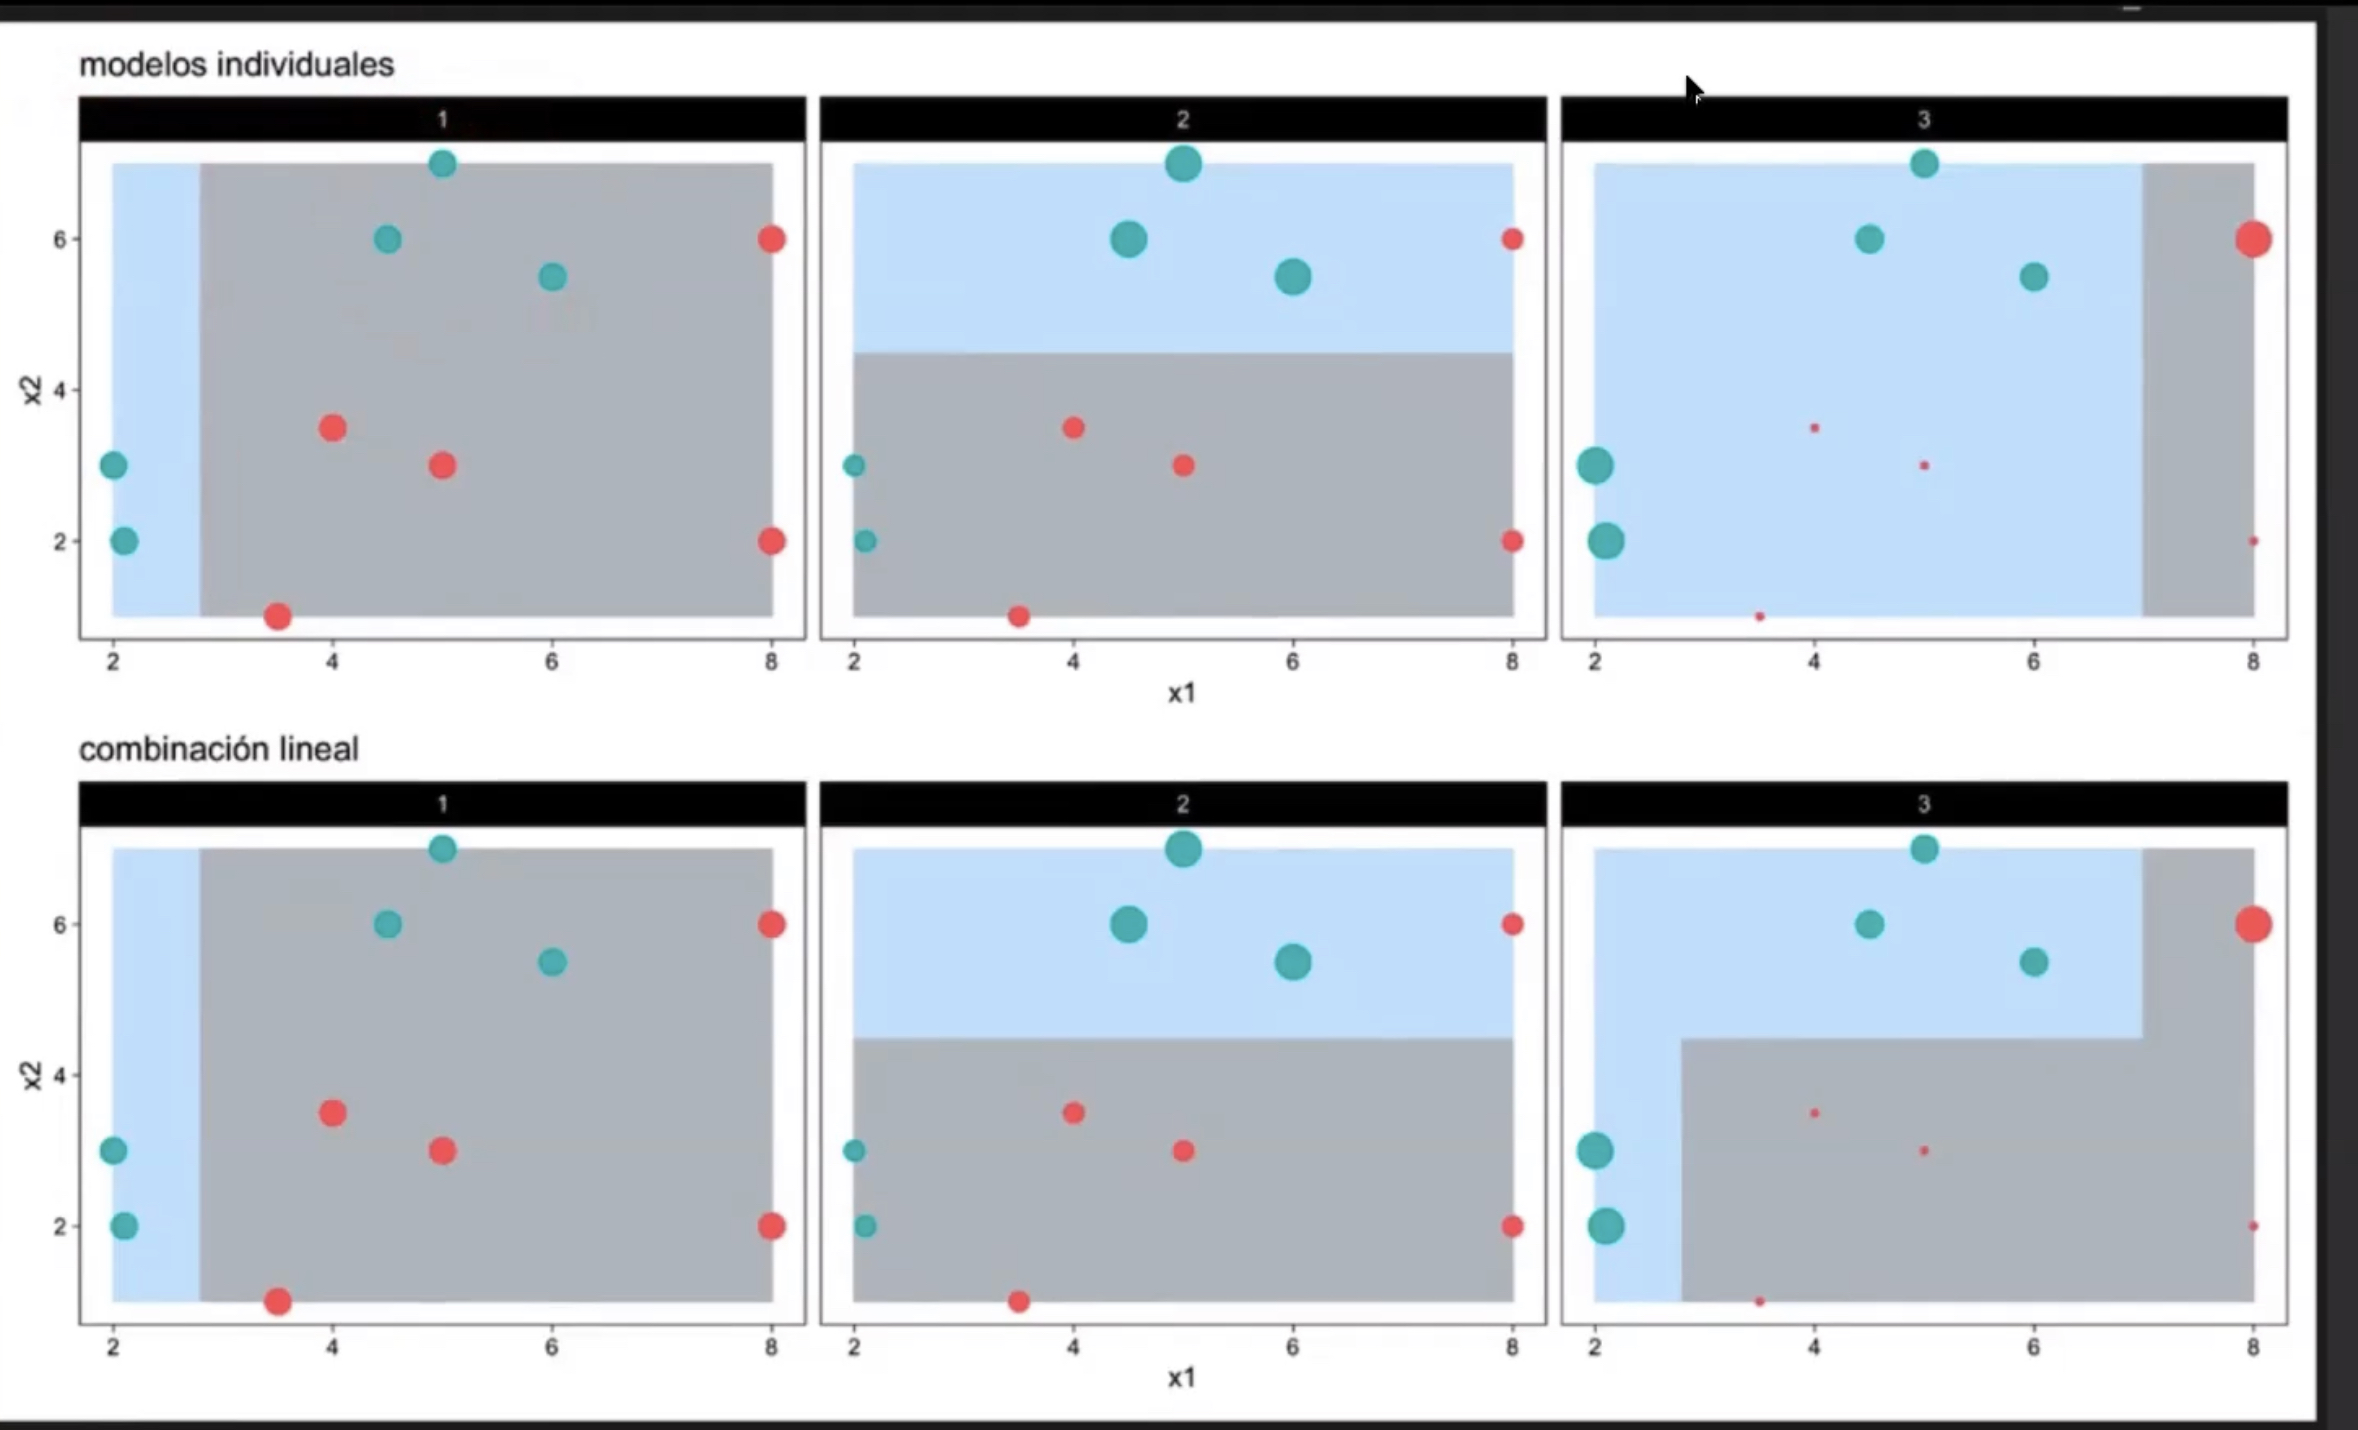
\includegraphics[width=0.8\textwidth]{Adaboost.jpeg}
    \caption{Modelos lineales vs. Combinación lineal}
    \label{fig:my_label}
\end{figure}
\begin{itemize}
    \item Los modelos débiles pueden fallar con probabilidad $\delta$. La probabilidad de éxito al tiempo T está acotada por $1-\delta T$
    \item ¿Como podemos garantizar que el error de estimación ($Ls(h_s) - \min_{h\in H} L_{\D}(h))$ es pequeño?\\
    $VCdim(H)\rightarrow pequeña \rightarrow$ garantiza buen desempeño
    \item $L(B,T)= \{h(x)= signo \left( \sum_{t=1}^T w_t h-t(x) \right) : x\in \R^d, wt \in \R^T, h_t \in R \}$
    \\
    $VCdim(L(B,T)) \leq T VCdim(B)$
    \\ Por lo tanto T nos ayuda a controlar el compromiso entre sesgo y varianza
\end{itemize}

\bibliographystyle{siam} % <<< USE "alpha" BIBLIOGRAPHY STYLE
\bibliography{template} % <<< RENAME TO "lecture_XX"


\end{document}
